\documentclass[oneside]{book}

% Creative Commons Attribution ShareAlike 4.0 https://creativecommons.org/licenses/by-sa/4.0/

\usepackage{fontspec}
\usepackage{fullpage}
\usepackage{hyperref}
\usepackage{multirow}
\usepackage[table]{xcolor}
\usepackage{tikz}
\usepackage[normalem]{ulem}

\newcommand{\LanguageName}{MyLang}
\newcommand{\LanguageCreator}{Your Name Here}

\hypersetup
{
    colorlinks=true,
    linkcolor=black,
    pdftitle={\LanguageName\ Reference by \LanguageCreator},
}

\begin{document}

\setmainfont[Ligatures=TeX]{DejaVu Sans}

\begin{center}
\Huge

{\ }

\vfil

\textsl{\LanguageName}

{\ }

\textsl{Reference Grammar}

\textsl{and Lexicon}

{\ }

{\ }

\Large

by \LanguageCreator

\vfil

{\ }
\end{center}

\vfil

\eject

\chapter{\LanguageName\ Language Description}

\section{Phonology}


\eject

\subsection{Consonants}

\LanguageName\ uses the following consonants.
In this abbreviated {\fontsize{8pt}{8pt}\selectfont IPA} table, any symbols on the left represent unvoiced consonants and any sounds on the right represent voiced consonants.

\begin{center}
\newcommand{\head}{\fontsize{7pt}{7pt}\selectfont}
\begin{tabular}{|r|cc|cc|cccccc|cc|cc|cc|cc|}\hline
&
\multicolumn{2}{|c|}{\head Bilabial}&
\multicolumn{2}{|c|}{\head Labiodental}&
\multicolumn{2}{|c|}{\head Dental}&
\multicolumn{2}{|c|}{\head Alveolar}&
\multicolumn{2}{|c|}{\head Postalveolar}&
\multicolumn{2}{|c|}{\head Retroflex}&
\multicolumn{2}{|c|}{\head Palatal}&
\multicolumn{2}{|c|}{\head Velar}&
\multicolumn{2}{|c|}{\head Glottal}\\\hline
\multirow{2}{*}{\head Plosive}&
\multirow{2}{*}{p}&
\multirow{2}{*}{b}&
&
&
&
&
\multirow{2}{*}{t}&
\multirow{2}{*}{d}&
&
&
\multirow{2}{*}{ʈ}&
\multirow{2}{*}{ɖ}&
\multirow{2}{*}{c}&
\multirow{2}{*}{ɟ}&
\multirow{2}{*}{k}&
\multirow{2}{*}{g}&
\multirow{2}{*}{ʔ}&
\cellcolor{gray}\\
&&&&&&&&&&&&&&&&&&\cellcolor{gray}\\\hline
\multirow{2}{*}{\head Nasal}&
&
\multirow{2}{*}{m}&
&
\multirow{2}{*}{ɱ}&
&
&
&
\multirow{2}{*}{n}&
&
&
&
\multirow{2}{*}{ɳ}&
&
\multirow{2}{*}{ɲ}&
&
\multirow{2}{*}{ŋ}&
\cellcolor{gray}&
\cellcolor{gray}\\
&&&&&&&&&&&&&&&&&\cellcolor{gray}&\cellcolor{gray}\\\hline
\multirow{2}{*}{\head Trill}&
&
\multirow{2}{*}{ʙ}&
&
&
&
&
&
\multirow{2}{*}{r}&
&
&
&
&
&
&
\cellcolor{gray}&
\cellcolor{gray}&
\cellcolor{gray}&
\cellcolor{gray}\\
&&&&&&&&&&&&&&&\cellcolor{gray}&\cellcolor{gray}&\cellcolor{gray}&\cellcolor{gray}\\\hline
\multirow{2}{*}{\head Fricative}&
\multirow{2}{*}{ɸ}&
\multirow{2}{*}{β}&
\multirow{2}{*}{f}&
\multirow{2}{*}{v}&
\multirow{2}{*}{θ}&
\multicolumn{1}{c|}{\multirow{2}{*}{ð}}&
\multicolumn{1}{c}{\multirow{2}{*}{s}}&
\multicolumn{1}{c|}{\multirow{2}{*}{z}}&
\multicolumn{1}{|c}{\multirow{2}{*}{ʃ}}&
\multirow{2}{*}{ʒ}&
\multirow{2}{*}{ʂ}&
\multirow{2}{*}{ʐ}&
\multirow{2}{*}{ç}&
\multirow{2}{*}{ʝ}&
\multirow{2}{*}{x}&
\multirow{2}{*}{ɣ}&
\multirow{2}{*}{h}&
\multirow{2}{*}{ɦ}\\
&&&&&\multicolumn{2}{c|}{}&\multicolumn{2}{c|}{}&\multicolumn{2}{|c|}{}&&&&&&&&\\\hline
{\head Lateral}&
\cellcolor{gray}&
\cellcolor{gray}&
\cellcolor{gray}&
\cellcolor{gray}&
&
&
\multirow{2}{*}{ɬ}&
\multirow{2}{*}{ɮ}&
&
&
&
&
&
&
&
&
\cellcolor{gray}&
\cellcolor{gray}\\
{\head fricative}&\cellcolor{gray}&\cellcolor{gray}&\cellcolor{gray}&\cellcolor{gray}&&&&&&&&&&&&&\cellcolor{gray}&\cellcolor{gray}\\\hline
\multirow{2}{*}{\head Approximant}&
&
&
&
\multirow{2}{*}{ʋ}&
&
&
&
\multirow{2}{*}{ɹ}&
&
&
&
\multirow{2}{*}{ɻ}&
&
\multirow{2}{*}{j}&
&
\multirow{2}{*}{ɰ}&
\cellcolor{gray}&
\cellcolor{gray}\\
&&&&&&&&&&&&&&&&&\cellcolor{gray}&\cellcolor{gray}\\\hline
{\head Lateral}&
\cellcolor{gray}&
\cellcolor{gray}&
\cellcolor{gray}&
\cellcolor{gray}&
&
&
&
\multirow{2}{*}{l}&
&
&
&
\multirow{2}{*}{ɭ}&
&
\multirow{2}{*}{ʎ}&
&
\multirow{2}{*}{ʟ}&
\cellcolor{gray}&
\cellcolor{gray}\\
{\head Approximant}&\cellcolor{gray}&\cellcolor{gray}&\cellcolor{gray}&\cellcolor{gray}&&&&&&&&&&&&&\cellcolor{gray}&\cellcolor{gray}\\\hline
\end{tabular}
\end{center}

For comparison, here are the consonants usually heard from in American English.

\begin{center}
\newcommand{\head}{\fontsize{7pt}{7pt}\selectfont}
\begin{tabular}{|r|cc|cc|cccccc|cc|cc|cc|cc|}\hline
&
\multicolumn{2}{|c|}{\head Bilabial}&
\multicolumn{2}{|c|}{\head Labiodental}&
\multicolumn{2}{|c|}{\head Dental}&
\multicolumn{2}{|c|}{\head Alveolar}&
\multicolumn{2}{|c|}{\head Postalveolar}&
\multicolumn{2}{|c|}{\head Retroflex}&
\multicolumn{2}{|c|}{\head Palatal}&
\multicolumn{2}{|c|}{\head Velar}&
\multicolumn{2}{|c|}{\head Glottal}\\\hline
\multirow{2}{*}{\head Plosive}&
\multirow{2}{*}{p}&
\multirow{2}{*}{b}&
&
&
&
&
\multirow{2}{*}{t}&
\multirow{2}{*}{d}&
&
&
&
&
&
&
\multirow{2}{*}{k}&
\multirow{2}{*}{g}&
&
\cellcolor{gray}\\
&&&&&&&&&&&&&&&&&&\cellcolor{gray}\\\hline
\multirow{2}{*}{\head Nasal}&
&
\multirow{2}{*}{m}&
&
&
&
&
&
\multirow{2}{*}{n}&
&
&
&
&
&
&
&
\multirow{2}{*}{ŋ}&
\cellcolor{gray}&
\cellcolor{gray}\\
&&&&&&&&&&&&&&&&&\cellcolor{gray}&\cellcolor{gray}\\\hline
\multirow{2}{*}{\head Trill}&
&
\multirow{2}{*}{ʙ}&
&
&
&
&
&
\multirow{2}{*}{r}&
&
&
&
&
&
&
\cellcolor{gray}&
\cellcolor{gray}&
\cellcolor{gray}&
\cellcolor{gray}\\
&&&&&&&&&&&&&&&\cellcolor{gray}&\cellcolor{gray}&\cellcolor{gray}&\cellcolor{gray}\\\hline
\multirow{2}{*}{\head Fricative}&
&
&
\multirow{2}{*}{f}&
\multirow{2}{*}{v}&
\multirow{2}{*}{θ}&
\multicolumn{1}{c|}{\multirow{2}{*}{ð}}&
\multicolumn{1}{c}{\multirow{2}{*}{s}}&
\multicolumn{1}{c|}{\multirow{2}{*}{z}}&
\multicolumn{1}{|c}{\multirow{2}{*}{ʃ}}&
&
&
&
&
&
&
&
\multirow{2}{*}{h}&
\\
&&&&&\multicolumn{2}{c|}{}&\multicolumn{2}{c|}{}&\multicolumn{2}{|c|}{}&&&&&&&&\\\hline
{\head Lateral}&
\cellcolor{gray}&
\cellcolor{gray}&
\cellcolor{gray}&
\cellcolor{gray}&
&
&
&
&
&
&
&
&
&
&
&
&
\cellcolor{gray}&
\cellcolor{gray}\\
{\head fricative}&\cellcolor{gray}&\cellcolor{gray}&\cellcolor{gray}&\cellcolor{gray}&&&&&&&&&&&&&\cellcolor{gray}&\cellcolor{gray}\\\hline
\multirow{2}{*}{\head Approximant}&
&
&
&
&
&
&
&
\multirow{2}{*}{ɹ}&
&
&
&
&
&
\multirow{2}{*}{j}&
&
&
\cellcolor{gray}&
\cellcolor{gray}\\
&&&&&&&&&&&&&&&&&\cellcolor{gray}&\cellcolor{gray}\\\hline
{\head Lateral}&
\cellcolor{gray}&
\cellcolor{gray}&
\cellcolor{gray}&
\cellcolor{gray}&
&
&
&
\multirow{2}{*}{l}&
&
&
&
&
&
&
&
\multirow{2}{*}{ʟ}&
\cellcolor{gray}&
\cellcolor{gray}\\
{\head Approximant}&\cellcolor{gray}&\cellcolor{gray}&\cellcolor{gray}&\cellcolor{gray}&&&&&&&&&&&&&\cellcolor{gray}&\cellcolor{gray}\\\hline
\end{tabular}
\end{center}

\eject

\subsection{Vowels}

\LanguageName\ uses the following vowels.
Any sounds before a dot (\textbullet) are pronounced with unrounded lips and any sounds after a dot are pronounced with rounded lips.
The vowels ə and ɐ do not specify lip shape and may be pronounced either way.

\begin{center}
\begin{tikzpicture}
\draw[ultra thick](0,6)--(4,0);
\draw[ultra thick](3.6,6)--(5.5,0);
\draw[ultra thick](7,6)--(7,0);
\draw[ultra thick](0.7,6)--(3,6);
\draw[ultra thick](4.5,6)--(5.9,6);
\draw[ultra thick](2,4)--(3.5,4);
\draw[ultra thick](5,4)--(6.3,4);
\draw[ultra thick](3.8,2)--(4.2,2);
\draw[ultra thick](5.6,2)--(6.3,2);
\draw[ultra thick](4.9,0)--(6.2,0);
\fill[white](4.3,2.7)rectangle(4.8,3.4);
\fill[white](4.9,0.7)rectangle(5.5,1.4);
\draw(0.1,6)node{\huge i\raisebox{-1.3mm}{\Huge\textbullet}y};
\draw(3.75,6)node{\huge ɨ\raisebox{-1.3mm}{\Huge\textbullet}ʉ};
\draw(6.9,5.9)node{\huge ɯ\raisebox{-1.3mm}{\Huge\textbullet} u};
\draw(2,5)node{\huge ɪ\raisebox{-1.3mm}{\Huge\textbullet}ʏ};
\draw(5.5,5)node{\huge\ \raisebox{-1.3mm}{\Huge\textbullet}ʊ};
\draw(1.3,3.95)node{\huge e\raisebox{-1.3mm}{\Huge\textbullet}ø};
\draw(4.25,3.95)node{\huge ɘ\raisebox{-1.3mm}{\Huge\textbullet}ɵ};
\draw(7,3.9)node{\huge ɤ\raisebox{-1.3mm}{\Huge\textbullet}o};
\draw(4.55,3)node{\huge ə};
\draw(2.85,1.95)node{\huge ɛ\raisebox{-1.3mm}{\Huge\textbullet}œ};
\draw(4.9,1.95)node{\huge ɜ\raisebox{-1.3mm}{\Huge\textbullet}ɞ};
\draw(7,1.95)node{\huge ʌ\raisebox{-1.3mm}{\Huge\textbullet}ɔ};
\draw(2.9,1)node{\huge æ\raisebox{-1.3mm}{\Huge\textbullet}\ };
\draw(5.2,1)node{\huge ɐ};
\draw(4.05,-0.05)node{\huge a\raisebox{-1.3mm}{\Huge\textbullet}ɶ};
\draw(7,-0.05)node{\huge ɑ\raisebox{-1.3mm}{\Huge\textbullet}ɒ};
\draw(0,6.8)node{Front};
\draw(3.5,6.8)node{Central};
\draw(7,6.8)node{Back};
\draw(-3,6)node[right]{Close};
\draw(-3,4)node[right]{Close-mid};
\draw(-3,2)node[right]{Open-mid};
\draw(-3,0)node[right]{Open};
\end{tikzpicture}
\end{center}

For comparison, here are the vowels usually heard in American English.

\begin{center}
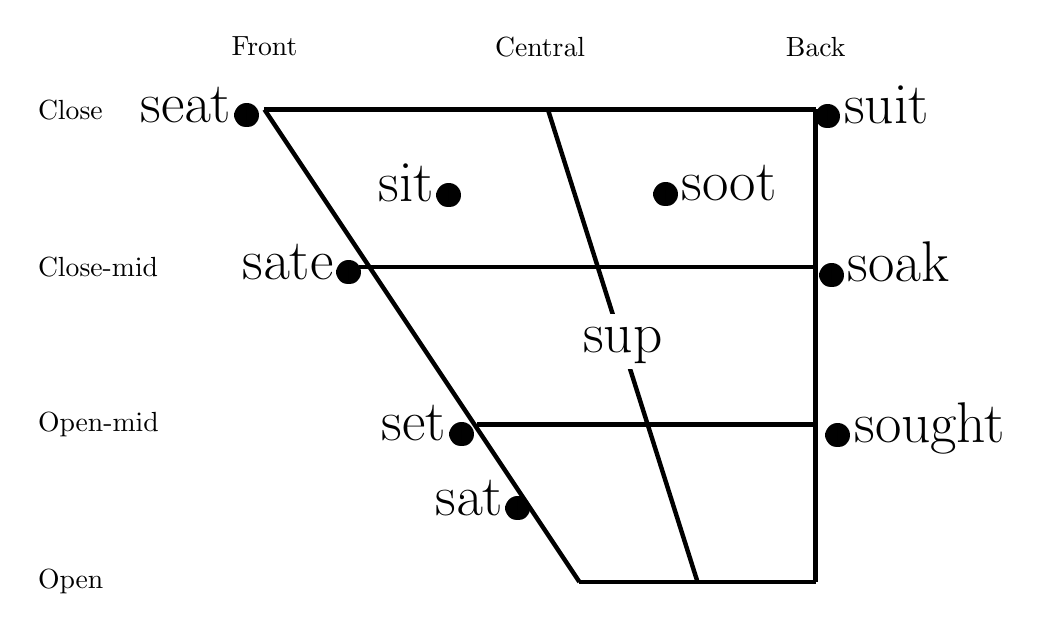
\begin{tikzpicture}
\draw[ultra thick](0,6)--(4,0);
\draw[ultra thick](3.6,6)--(5.5,0);
\draw[ultra thick](7,6)--(7,0);
\draw[ultra thick](0,6)--(7,6);
\draw[ultra thick](1.2,4)--(7,4);
\draw[ultra thick](2.7,2)--(7,2);
\draw[ultra thick](4,0)--(7,0);
\fill[white](4.3,2.7)rectangle(4.8,3.4);
\draw(-0.8,6)node{\huge seat\raisebox{-1.3mm}{\Huge\textbullet}};
\draw(7.7,6)node{\huge\raisebox{-1.3mm}{\Huge\textbullet}suit};
\draw(2,5)node{\huge sit\raisebox{-1.3mm}{\Huge\textbullet}};
\draw(5.7,5)node{\huge\raisebox{-1.3mm}{\Huge\textbullet}soot};
\draw(0.5,4)node{\huge sate\raisebox{-1.3mm}{\Huge\textbullet}};
\draw(7.85,4)node{\huge\raisebox{-1.3mm}{\Huge\textbullet}soak};
\draw(4.55,3)node{\huge sup};
\draw(2.1,1.95)node{\huge set\raisebox{-1.3mm}{\Huge\textbullet}};
\draw(8.25,1.95)node{\huge\raisebox{-1.3mm}{\Huge\textbullet}sought};
\draw(2.8,1)node{\huge sat\raisebox{-1.3mm}{\Huge\textbullet}};
\draw(0,6.8)node{Front};
\draw(3.5,6.8)node{Central};
\draw(7,6.8)node{Back};
\draw(-3,6)node[right]{Close};
\draw(-3,4)node[right]{Close-mid};
\draw(-3,2)node[right]{Open-mid};
\draw(-3,0)node[right]{Open};
\end{tikzpicture}
\end{center}

\subsection{Tone}

[[If the language has lexical tone, state whether it’s register or contour, then list either all the tones, or all the tone melodies.
Also make a note if tone is used grammatically.]]

\subsection{Stress}

[[If the language has stress, list the stress rules here, with examples if necessary.]]

\section{Writing}

\subsection{Transcription}

The symbols listed in the tables above are phonetic symbols.
These will be used to \emph{transcribe} \LanguageName\ words, but not to \emph{write} them.
To write them, we utilize a romanization system that should make the pronunciation fairly transparent.
That transcription system is listed below:

\begin{itemize}
\item
The following sounds will be written using the same letter as their phonetic symbol:
\textbf{p}, \textbf{b}, \textbf{w}, \textbf{m}, \textbf{n}, \textbf{s}, \textbf{z}, \textbf{l}, \textbf{k}, \textbf{g}, \textbf{t}, \textbf{d}, \textbf{ts}, \textbf{dz}, \textbf{q}, \textbf{i}, \textbf{e}, \textbf{u}, \textbf{o}, \textbf{ǝ} and \textbf{a}.
\item
The sounds [tʃ] (kind of like the ``ch'' in ``\uline{ch}arge'') will be spelled \textbf{ch}.
\item
The sounds [dʒ] (kind of like the ``j'' in ``\uline{j}ar'') will be spelled \textbf{j}.
\item
The sound [ʝ] (similar to the ``z'' in ``a\uline{z}ure'') will be spelled \textbf{zh}.
\item
The sound [ɖ] (no English equivalent) will be spelled \textbf{d}.
\item
The sounds [ɟ] and [ʝ] (kind of like the ``j'' in ``\uline{j}ar'') will be spelled \textbf{j}.
\item
The sound [j] (like the ``y'' in ``\uline{y}ellow'') will be spelled \textbf{y}.
\item
The sound [ç] (like the ``h'' in ``\uline{h}eat'') will be spelled \textbf{hy}.
\item
The sound [ʍ] (like the ``wh'' in old pronunciations of ``\uline{wh}ich'') will be spelled \textbf{hw}.
\item
The sound [ŋ] (like the ``ng'' in ``si\uline{ng}'') will be spelled \textbf{ng}.
\item
The sound [ɲ] (like the ``ni'' in ``o\uline{ni}on'') will be spelled \textbf{ny}.
\item
The sound [ɴ] (no English equivalent) will be spelled \textbf{n} when occurring before uvular consonants.
\item
The sound [θ] (like the ``th'' in ``\uline{th}in'') will be spelled \textbf{th}.
\item
The sound [ð] (like the ``th'' in ``\uline{th}is'') will be spelled \textbf{dh}.
\item
The sound [ʃ] (like the ``sh'' in ``\uline{sh}e'') will be spelled \textbf{sh}.
\item
The sound [ʒ] (like the ``z'' in ``a\uline{z}ure'') will be spelled \textbf{zh}.
\item
The sounds [ɣ] and [ʁ] (no English equivalent) will be spelled \textbf{gh}.
\item
The sound [ɢ] (no equivalent in any well-known languages) will be spelled \textbf{qg}.
\item
The sound [ħ] (no English equivalent; sounds a bit like fogging up a mirror) will be spelled \textbf{h}.
\item
The sounds [x] and [χ] (like the ``ch'' Scottish ``lo\uline{ch}'') will be spelled \textbf{kh}.
\item
The sound [ɾ] (like the ``t'' or ``d'' in ``ma\uline{t}a\uline{d}or'') will be spelled \textbf{r}.
\item
The sound [r] (like the ``rr'' in Spanish ``pe\uline{rr}o'') will be spelled \textbf{r}.
\item
The sound [ʔ] (like the ``-'' in ``uh\uline{-}oh'') will be spelled \textbf{'}.
\item
The sound [ʕ] (no English equivalent; sounds a bit like gagging) will be spelled \textbf{'} (i.e. with an apostrophe).
\item
The sound [ɑ] (like the ``a'' in ``f\uline{a}ther'') will be spelled \textbf{a}.
(\emph{Note:} For the sake of simplicity, the sound [ɑ] will be transcribed [a] in the phonetic transcriptions below.)
\item
The sound [ɛ] (like the ``e'' in ``g\uline{e}t'') will be spelled \textbf{e}.
(\emph{Note:} For the sake of simplicity, the sound [ɛ] will be transcribed [e] in the phonetic transcription given in the relevant entries below.)
\item
The sound [e] (like the ``e'' in ``h\uline{e}y'') will be spelled \textbf{ei}.
\item
The sound [æ] (like the ``a'' in ``b\uline{a}d'') will be spelled \textbf{a}.
\item
The sound [ɪ] (like the ``i'' in ``k\uline{i}d'') will be spelled \textbf{i}.
\item
The sound [ɨ] (like the ``e'' in ``ch\uline{i}cken'') will be spelled \textbf{i}.
\item
The sound [ɔ] (like the ``aw'' in ``l\uline{aw}'') will be spelled \textbf{o}.
\item
The sound [œ] (no English equivalent; like the ``ö'' in German ``hören'') will be spelled \textbf{ö}.
(\emph{Note:} For the sake of simplicity, the sound [œ] will be transcribed [ø] in the phonetic transcription given in the relevant entries below.)
\item
The sound [y] (no English equivalent; like the ``ü'' in German ``für'') will be spelled \textbf{ü}.
\item
The sound [ɤ] (like the ``o'' in ``st\uline{o}ke'', but with the lips left unrounded) will be spelled \textbf{ë}.
\item
The sound [o] (like the ``o'' in ``r\uline{o}te'') will be spelled \textbf{ou}.
\item
The sound [ʊ] (like the ``oo'' in ``w\uline{oo}d'') will be spelled \textbf{u}.
\item
The sound [ɯ] (like the ``u'' in ``r\uline{u}ne'', but with the lips left unrounded) will be spelled \textbf{ï}.
\item
The sound [ǝ] (like the ``a'' in ``sof\uline{a}'') will be spelled \textbf{a}.
Long vowels will be written with a doubled version of the vowel (so [iː] will be written \textbf{ii}).
\end{itemize}

\subsection{Romanization}

This is the romanization system, which will be used to spell the language using the Roman alphabet.
This is also how to find \LanguageName\ words in the \LanguageName-English dictionary.
The full system is described in detail below:

\begin{itemize}
\item
\textbf{A}, \textbf{a}:
Pronounced like the ``\uline{a}'' in ``f\uline{a}ther''.
\item
\textbf{Aa}, \textbf{aa}:
Pronounced like the ``\uline{a}'' in ``f\uline{a}ther'', but held slightly longer.
\item
\textbf{B}, \textbf{b}:
Pronounced like the ``\uline{b}'' in ``\uline{b}ad''.
\item
\textbf{Ch}, \textbf{ch}:
Pronounced like the ``\uline{ch}'' in ``ea\uline{ch}''.
Unlike the sound ``\uline{ch}'' in English ``\uline{ch}air'', there is no discernible puff of air that accompanies this sound.
If one holds one's breath while pronouncing the ``\uline{ch}'' in English ``\uline{ch}air'', one will pronounce this sound correctly.
\item
\textbf{D}, \textbf{d}:
Pronounced like the ``\uline{d}'' in ``\uline{d}iet''.
\item
\textbf{Dz}, \textbf{dz}:
Pronounced like the ``\uline{ds}'' in ``mo\uline{ds}''.
\item
\textbf{E}, \textbf{e}:
Pronounced like the ``\uline{e}'' in ``g\uline{e}t''.
\item
\textbf{Ǝ}, \textbf{ǝ}:
Pronounced like the ``\uline{a}'' in ``sof\uline{a}''.
\item
\textbf{F}, \textbf{f}:
Pronounced like the ``\uline{f}'' in ``\uline{f}og''.
\item
\textbf{G}, \textbf{g}:
Pronounced like the ``\uline{g}'' in ``\uline{g}oat'' (never like the ``\uline{g}'' in ``\uline{g}enius'').
\item
\textbf{Gh}, \textbf{gh}:
Pronounced like the ``\uline{r}'' in French ``\uline{r}ouge'' (never like the ``\uline{gh}'' in ``\uline{gh}ost'').
\item
\textbf{I}, \textbf{i}:
Pronounced like the ``\uline{i}'' in ``mach\uline{i}ne''.
\item
\textbf{Ii}, \textbf{ii}:
Pronounced like the ``\uline{i}'' in ``mach\uline{i}ne'', but held slightly longer.
\item
\textbf{J}, \textbf{j}:
Pronounced like the ``\uline{j}'' in ``\uline{j}am''.
\item
\textbf{K}, \textbf{k}:
Pronounced like the ``\uline{k}'' in ``s\uline{k}y'' (this sound features no aspiration.
Aspiration is the puff of air that occurs in the ``\uline{k}'' in ``\uline{k}ite''.
Compare the ``\uline{k}'' in ``\uline{k}ite'' and the ``\uline{k}'' in ``s\uline{k}y'' [try holding your hand in front of your face when pronouncing both].
The \LanguageName\ \textbf{k} should always be pronounced like the ``\uline{k}'' in ``s\uline{k}y'';
never like the ``\uline{k}'' in ``\uline{k}ite'').
\item
\textbf{K'}, \textbf{k'}:
There's no English equivalent to this sound.
This is an ejective consonant.
In the case of \textbf{k'}, it's pronounced just like \textbf{k}, but with one's breath held.
The result is a little ``popping'' sound that immediately follows the production of the \textbf{k}.
You can think of it as a \textbf{k} that's followed by a glottal \textbf{'} sound.
Producing those two sounds in short succession will result in a sound very close to \textbf{k'}.
Continue to practice and you should be able to get it.
\item
\textbf{Kh}, \textbf{kh}:
Pronounced like the ``\uline{ch}'' in the German pronunciation of ``Bu\uline{ch}''.
In English, this sound is commonly used with onomatopoeic words associated with disgust, like ``ble\uline{ch}!'' or ``i\uline{ch}!''
To pronounce it correctly, put your tongue in position to pronounce a \textbf{k}, but release it slowly;
allow the air to pass through the constricted space.
The result should be a sound like white noise.
\item
\textbf{L}, \textbf{l}:
Pronounced like the ``\uline{l}'' in ``\uline{l}ove''.
\item
\textbf{M}, \textbf{m}:
Pronounced like the ``\uline{m}'' in ``\uline{m}atter''.
\item
\textbf{N}, \textbf{n}:
Pronounced like the ``\uline{n}'' in ``\uline{n}ever''.
\item
\textbf{Ng}, \textbf{ng}:
Pronounced like the ``\uline{ng}'' in ``si\uline{ng}''.
\item
\textbf{O}, \textbf{o}:
Pronounced like the ``\uline{o}'' in ``t\uline{o}te''.
\item
\textbf{Ö}, \textbf{ö}:
Pronounced like the ``\uline{œu}'' in French ``s\uline{œu}r'', or the ``\uline{ö}'' in German ``h\uline{ö}ren''.
\item
\textbf{P}, \textbf{p}:
Pronounced like the ``\uline{p}'' in ``s\uline{p}ike'' (this sound features no aspiration.
Aspiration is the puff of air that occurs in the ``\uline{p}'' in ``\uline{p}ike''.
Compare the ``\uline{p}'' in ``\uline{p}ike'' and the ``\uline{p}'' in ``s\uline{p}ike'' [try holding your hand in front of your face when pronouncing both].
The \LanguageName\ \textbf{p} should always be pronounced like the ``\uline{p}'' in ``s\uline{p}ike'';
never like the ``\uline{p}'' in ``\uline{p}ike'').
\item
\textbf{Q}, \textbf{q}:
This is likely the most difficult sound in \LanguageName\ for an English speaker to master.
The sound is produced by touching the back of the tongue to the uvula and making a constriction as one would for a \textbf{k}.
One pronounces this sound like any other stop (\textbf{p}, \textbf{t}, \textbf{k}), it's just pronounced further back in the mouth than an English speaker is used to.
Think about when the doctor asks you to go, ``Ahhhhhhh$\ldots$''
Try doing that, and as you're doing it, take the back of your tongue, without moving it, and plug up the opening in the back of your mouth.
That should put you in perfect position to pronounce \textbf{q}.
\item
\textbf{R}, \textbf{r}:
Pronounced like the ``\uline{r}'' in Spanish ``pe\uline{r}o''.
Nearly identical to the ``\uline{t}'' or ``\uline{d}'' sound in English ``ma\uline{t}a\uline{d}or'' (pronounced quickly).
\item
\textbf{S}, \textbf{s}:
Pronounced like the ``\uline{s}'' in ``\uline{s}ad''.
\item
\textbf{Sh}, \textbf{sh}:
Pronounced like the ``\uline{sh}'' in ``\uline{sh}ade''.
\item
\textbf{T}, \textbf{t}:
Pronounced like the ``\uline{t}'' in ``s\uline{t}ake'' (this sound features no aspiration.
Aspiration is the puff of air that occurs in the ``\uline{t}'' in ``\uline{t}ake''.
Compare the ``\uline{t}'' in ``\uline{t}ake'' and the ``\uline{t}'' in ``s\uline{t}ake'' [try holding your hand in front of your face when pronouncing both].
The \LanguageName\ \textbf{t} should always be pronounced like the ``\uline{t}'' in ``s\uline{t}ake'';
never like the ``\uline{t}'' in ``\uline{t}ake'').
\item
\textbf{Ts}, \textbf{ts}:
Pronounced like the ``\uline{ts}'' in ``cu\uline{ts}''.
\item
\textbf{U}, \textbf{u}:
Pronounced like the ``\uline{u}'' in ``r\uline{u}minate''.
\item
\textbf{Uu}, \textbf{uu}:
Pronounced like the ``\uline{u}'' in ``r\uline{u}minate'', but held slightly longer.
\item
\textbf{Ü}, \textbf{ü}:
Pronounced like the ``\uline{u}'' in French ``r\uline{u}e'', or the ``\uline{ü}'' in German ``f\uline{ü}r''.
\item
\textbf{Üü}, \textbf{üü}:
Pronounced like the ``\uline{u}'' in French ``r\uline{u}e'', or the ``\uline{ü}'' in German ``f\uline{ü}r'', but held slightly longer.
\item
\textbf{V}, \textbf{v}:
Pronounced like the ``\uline{v}'' in ``\uline{v}an''.
\item
\textbf{W}, \textbf{w}:
Pronounced like the ``\uline{w}'' in ``\uline{w}alk''.
\item
\textbf{Y}, \textbf{y}:
Pronounced like the ``\uline{y}'' in ``\uline{y}et''.
\item
\textbf{Z}, \textbf{z}:
Pronounced like the ``\uline{z}'' in ``\uline{z}ebra''.
\item
\textbf{Zh}, \textbf{zh}:
Pronounced like the ``\uline{z}'' n ``a\uline{z}ure''.
\item
\textbf{'}:
This is referred to as a glottal stop, and is pronounced just like the catch in one's throat that occurs in between the ``uh'' and ``oh'' in English ``uh\uline{-}oh''.
This isn't a difficult sound to produce;
it just requires a bit of practice to insert it into words.
It will occur naturally in a string of vowels pronounced separately in English (e.g. if one were to say ``A A A A A A A'' [saying the actual name of the letter each time] over and over, a glottal stop will naturally occur before each instance of the vowel).
If one simply stops pronouncing a word mid-vowel and starts again, it will naturally occur.
(Note: It is important to remember that this apostrophe is not a stray mark, and not simply there for decoration.
The apostrophe stands for a consonant which has the same status as \textbf{g} or \textbf{k} or any other consonant.)
\item
\textbf{Double Consonants:}
Doubled consonants, or geminates, occur frequently in \LanguageName.
To pronounce a doubled consonant, simply pronounce it twice.
You might think of it as lingering over the consonant.
Think of the ``\uline{s}'' sound you pronounce in ``Mi\uline{ss S}ally''.
It's a longer ``\uline{s}'' than if you pronounce the similar phrase ``Mi\uline{ss} Ally''.
The same goes for the doubled consonants of \LanguageName.
One important note about the romanization:
If a digraph (e.g. \textbf{kh}, \textbf{gh}, etc.) is doubled, only the first letter will be doubled (hence, \textbf{kkh} not \textbf{khkh}).
The consonant is pronounced like a doubled consonant, though, as actual combinations such as \textbf{k} followed by \textbf{kh} are impossible.
\end{itemize}

\subsection{Orthography}

\LanguageName\ has a unique orthography used to write it.
The font face is called \texttt{\LanguageName-Regular.ttf}.
Below is a short description of how it is used:

\begin{itemize}
\item
Å is used for \textbf{'}, the glottal stop.
It also doubles as the vowel \textbf{a}.
It is used in conjunction with \textbf{Ŷ} to form the vowel \textbf{e} (i.e. e), and used in conjunction with \textbf{Ù} to form the vowel \textbf{o} (i.e. o).
\item
ß is used for \textbf{b}.
\item
Ç is used for \textbf{ch}.
Note that this is a combination of \textbf{ts} (i.e. Ž) and \textbf{y} (i.e. Ŷ).
Note that there is no character used for \textbf{ǝ}.
For the orthographic number system of NewLang, see the section on numbers below.
\end{itemize}

\section{Morphology and Syntax}

\LanguageName\ is a [[list dominant word order (SVO / $\ldots$) and level of synthesis (isolating / agglutinating / fusional / polysythetic).
List order of noun-adjective, noun-genetive, adposition-noun, and noun-relative clause]].

\subsection{Nouns}

NewLang nouns [[state whether nouns inflect for number, case, gender, or possessive status.
If they do, list which categories are relevant for each]].

\begin{itemize}
\item
\textbf{Noun Function:}
[[State how you know who does what to whom, even if it's word order.
This section may be renamed Noun Case.]]
\item
\textbf{Noun Number:}
[[State how number works.]]
\item
\textbf{Noun Gender:}
[[State which genders are present and how they're reified.]]
\item
\textbf{Noun Possession:}
[[If not already indicate, state how noun possession works.]]
\end{itemize}

\subsection{Adjectives}

\LanguageName\ adjectives [[state how adjectives work, including whether or not they agree with nouns in case, number, or gender, and if they inflect for degree of comparison.
If there are no adjectives, delete this section.]]:

\begin{itemize}
\item
\textbf{Adjective Placement:}
[[Show how adjectives work when modifying a noun, and state if it's possible to have predicative adjectives.]]
\item
\textbf{Adjectival Agreement:}
[[Show how adjectival agreement works, if adjectives agree with nouns.]]
\item
\textbf{Comparison:}
[[Show how adjectives inflect or otherwise showcase comparison.
If not relevant, delete.]]
\end{itemize}

\subsection{Demonstratives}

[[State various types of demonstratives in \LanguageName.
Usually it1ll be deictic demonstratives, but there may be a reason to include others.
What demonstratives there are, state how the relevant categories work with respect to those demonstratives (e.g. case, number, gender).]]

\subsection{Verbs}

NewLang verbs [[state whether verbs conjugate for tense, aspect, modality, voice, or polarity.
State whether verbs agree with anything.
State whatever else is relevant in a top-level introduction to verbs]]:

\begin{itemize}
\item
\textbf{Copula:}
[[State how copular constructions work, even if there is no copula.]]
\item
\textbf{Negation:}
[[State how negation works.]]
\item
\textbf{Participles:}
[[You know, why not$\ldots$
If there are participles, put them here.]]
\end{itemize}

\subsection{Adverbs}

There are three types of adverbs:
manner, locational, and temporal.
[[State where adverbs occur.
If there's an obvious derivation connection between manner adverbs and adjectives, maybe mention that]]:

\subsection{Coordination}

[[State how coordination works.]]

\subsection{Relative Clauses}

[[State how relative clauses work, then show examples of the various types]]:

\begin{tabular}{lll}
\textbullet&\textbf{Subject:}&example \uline{that} you know.\\
&&\textbf{Example \uline{that} you know.}\\
&&``Example \uline{that} you know.''\\
\textbullet&\textbf{Direct Object:}&example \uline{that} you know.\\
&&\textbf{Example \uline{that} you know.}\\
&&``Example \uline{that} you know.''\\
\textbullet&\textbf{Indirect Object:}&example \uline{that} you know.\\
&&\textbf{Example \uline{that} you know.}\\
&&``Example \uline{that} you know.\\
\textbullet&\textbf{Adposition Object:}&example \uline{that} you know.\\
&&\textbf{Example \uline{that} you know.}\\
&&``Example \uline{that} you know.\\
\textbullet&\textbf{Possesive:}&example \uline{that} you know.\\
&&\textbf{Example \uline{that} you know.}\\
&&``Example \uline{that} you know.\\
\end{tabular}

\subsection{Questions}

\textbf{Yes/No Questions:}
[[State how yes/no questions work, and show examples.
Probably good to do negative yes/no questions too.]]

\textbf{WH-Questions:}
WH-questions are so called because in English, most WH-questions feature a word that has ``w'' and ``h'' in it (i.e. \uline{wh}o, \uline{wh}y, \uline{wh}at, \uline{wh}ere, \uline{wh}en or \uline{h}o\uline{w} [or even \uline{wh}ich]).
[[State how WH-questions work briefly, then given an example of each below.]]
Examples are given below:

\begin{tabular}{llll}
\textbullet&\textbf{Who:}&example \uline{what}?&(Test)\\
&&\textbf{Example \uline{what}?}\\
&&``Example \uline{what}?''\\
\textbullet&\textbf{What:}&example \uline{what}?&(Test)\\
&&\textbf{Example \uline{what}?}\\
&&``Example \uline{what}?''\\
\textbullet&\textbf{Where:}&example \uline{what}?&(Test)\\
&&\textbf{Example \uline{what}?}\\
&&``Example \uline{what}?''\\
\textbullet&\textbf{When:}&example \uline{what}?&(Test)\\
&&\textbf{Example \uline{what}?}\\
&&``Example \uline{what}?''\\
\textbullet&\textbf{How:}&example \uline{what}?&(Test)\\
&&\textbf{Example \uline{what}?}\\
&&``Example \uline{what}?''\\
\textbullet&\textbf{Which:}&example \uline{what}?&(Test)\\
&&\textbf{Example \uline{what}?}\\
&&``Example \uline{what}?''\\
\textbullet&\textbf{Whose:}&example \uline{what}?&(Test)\\
&&\textbf{Example \uline{what}?}\\
&&``Example \uline{what}?''\\
\textbullet&\textbf{How Many:}&example \uline{what}?&(Test)\\
&&\textbf{Example \uline{what}?}\\
&&``Example \uline{what}?''\\
\textbullet&\textbf{Why:}&example \uline{what}?&(Test)\\
&&\textbf{Example \uline{what}?}\\
&&``Example \uline{what}?''\\
\end{tabular}

\section{Historical Notes}

Below is a behind-the-scenes description of the historical processes that gave rise to the alternations seen in \LanguageName.
In the descriptions below, a segment, word or phrase preceded by an asterisk (*) is a proto-form.
A proto-form is an older form that's no longer present in the modern language.
[[List all of the sound changes in order.]]

\begin{itemize}
\item
\textbf{Loss of Schwa:}
*ǝ > Ø / \_,G

The basic schwa was lost next to glides and the glottal stop.
These sounds affected a change in the surrounding vowels, resulting in modern i, u, and a, as well as older *ai and *au.
\item
\textbf{Loss of Diphthongs:}
*ai, *au > e, o

diphthongs *ai and *au became e and o, respectively.
\item
\textbf{Schwa Lowering:}
*ǝ > a / \{C[+back], G\}\_

Schwa lowered to a when it followed q,kh, gh, w, y or ‘.
\item
\textbf{Vowel Lowering:}
*i, *u > e, o / [+back]\_

Vowels lowered when they followed q,kh, gh, or ‘.
\item
\textbf{Stop Insertion:}
Ø > C[-cont] / N\_L

A homorganic stop is inserted inbetween a nasal and a liquid.
\item
\textbf{Nasal Assimilation:}
N > [αplace] / \_,C[αplace]

Nasals assimilate in place to a following or preceding consonant, with few exceptions.
One exception is the velar nasal, which doesn't assimilate in place to a following consonant unless that consonant is y.
Other exceptions will be noted when they occur.
\item
\textbf{Vowel Fronting:}
V[-low] > [+front] / V[+front]...\_\#

In many instances, the vowels u and o fronted to ü and ö respectively when occurring after the vowels i, ü, ö or e.
This only happened when there were no other intervening vowels or glottalic consonants (t', ts', k', q', ', *b', *d'), and preferentially in closed syllables.
Also, it only occurred with *e (not *ai).
\item
\textbf{Vowel Devoicing:}
V > [-voice] / C[+CG]\_C[-voice]

Vowels devoice in between ejectives and voicelesssounds.
\item
\textbf{Progressive Voicing Assimilation:}
C > [αvoice] / \_C[αvoice]

Generally a consonant takes on the voicing of the one followingit.
\item
\textbf{Back Vowel Lenition:}
V[+back, -low] > v / \_V

Where ordinarily vowel hiatus would result in either a diphthong or two vowel nuclei separated by a glottal stop, non-low back vowels instead become the semi-vowel/fricative v.
This occurs, for example, when the perfect prefix k'u- occurs directly before a vowel-initial verbal stem other than u or ü.
\item
\textbf{Loss of Implosives:}

All implosives becameand *d' > d.
simple voiced plosives in all environments: *b' > b,
\item
\textbf{Affricate Gemination:}

Sequences of affricates become a single affricate with a geminate onset: tsts > tts, dzdz > ddz, ts'ts' > tts'.
\item
\textbf{Word-Final Stop Simplification:}
*C[+stop] > [-voice, -CG] / \_\#

All stops became plain voiceless stops at the end of a word.
(Note that q' becomes k at the end of a word.)
\item
\textbf{Compensatory Lengthening:}
*V > Vː / \_C[+voice]

All vowels lengthened before word-final voiced obstruents that became voiceless as a result of the previous change.
Prominent vowels in diphthongs became long, destroying the on- and off-glide-like vowels in the process.
\item
\textbf{Glottalic Dissimilation:}
C > [-glottalic] / C[+glottalic]V\_

This rule prevents consecutive ejectives from occurring in the language.
\item
\textbf{Loss of Voiced Velar Stop:}
*g > ng

This was a ubiquitous sound change.
\item
\textbf{Loss of Long Mid Vowels:}
*ey, *ee > ii; *ow, *oo > uu

This was a ubiquitous sound change.
\item
\textbf{Diphthong Simplification:}
*aw > o; *ew > u; *ay > e; *oy > i / \_, Stress; *uw > uu; *iy > ii

A diphthong will become the corresponding monophthong when it is unstressed.
The latter two changes affecting a sequence of a high vowel followed by a glide occur in all instances.
\item
\textbf{Nasal Assimilation:}
C[+nasal] > [αplace] / \_C[αplace]

This happened with all nasals.
\item
\textbf{Fortition:}
V > Vː / \_k', ch', t', ', h, w, y; t, k, s, sh, kh, l, m, n, ng, ny, b, d, j > tt, kk, ss, ssh, kkh, ll, mm, nn, nng, nny, bb, dd, jj

Stressed syllables strengthen either by lengthening the vowel or doubling the coda consonant.
What happens with each specific coda consonant is shown above.
\item
\textbf{Lenition:}
*t', *ch', *k', *t, *ch, *k, *b, *d, *j, *kh, *h > t, ch, k, d, j, *g, m, n, ny, Ø, Ø

Lenition occurs outside of the first syllable at the head of a strong syllable (stressed CVC syllable).
To give an example, with an underlying form like /tak-u-n-s/, the result would be takkunaas.
With an underlying form like /tak-tak-u-n-s/, though, the result would be tattagunnas, with the underlying /k/ leniting to g (note: this sound later changed to ng, so the final form would be tattangunnas).
\item
\textbf{Devoicing:}
C[+obs] > [-voice] / \_C[-voice]

The voiced obstruents *z, *v, *b, *d and *g devoice to s, f, p, t and k respectively when occurring before s, h, p, t and k.
Also, *z devoices to s in word-final position.
\item
\textbf{Voicing:}
C > [+voice] / C[+nasal]\_, \_C[+voice, -cont]

The voiceless stops *p, *t and *k voice to b, d and g after nasals and before b, d and g.
\item
\textbf{Fortition I:}
C > [+stop] / C[+nasal]\_

The fricatives/approximants *v, *z, *l, *r and *s all become stops when occurring after nasals.
The fricative *v becomes b after nasals, and the other consonants become d.
(Important note: This sound change continues to occur, and is applied again after the last rule listed here.)
\item
\textbf{Fortition II:}
C[+lateral] > [+stop] / \_V[+high]

The approximants *l and *r become d when occurring directly before u or i.
Note that this does not occur if the vowel has resulted from a sequence whose first vowel wasn't high and which occurred as a result of glide simplification (see below).
\item
\textbf{Glottal Deletion I:}
C[+glottal] > Ø / V\_V[-back], \_\#

The voiceless fricative h disappears after a vowel and before i or e.
The h is retained if the vowels are identical.
The consonant h is always lost word-finally, though (occasionally reappearing if the word comes before another that begins with a vowel).
\item
\textbf{Glottal Deletion II:}
C[+glottal] > Ø / C[+obs]\_

The voiceless fricative h disappears after stops,fricatives and approximants.
\item
\textbf{Hiatus:}
VV > CV, V

The following happens when two vowels come into contact:
*aa, *ea, *oa > a; *ii, *ei > i; *uu, *eu, *ou > u; *au, *ao > o; *ai, *ae, *oi > e; *ia > ya; *ua > wa; *ie > ye; *ue > we; *io > yo; *uo > wo; *iu > yu; *ui > wi.
\item
\textbf{Glide Gemination:}
Cx[+glide]Cx[+glide] > [+continuant]

When two glides come into contact with one another, it produces the following results:
*ww > v; *yy > j; *hh > h.
Note that the latter rule applies even in situations where h would ordinarily be deleted (see above).
\end{itemize}

\chapter{\LanguageName\ Reference Grammar}

\section{Personal Pronouns}

\begin{center}
\begin{tabular}{|l|l|l|}\hline
&\textbf{Singular}&\textbf{Plural}\\\hline
\textbf{First Person}&I&We\\\hline
\textbf{Second Person}&You&Youse\\\hline
\textbf{Third Person}&Ey&They\\\hline
\end{tabular}
\end{center}

\section{Nouns}

\subsection{Nominal Inflection}

\textbf{Word} \textit{``meaning''}, \textbf{wordy} \textit{``meaning''}

\begin{center}
\begin{tabular}{|l|l|l|l|l|l|l|}\hline
&\multicolumn{3}{|c|}{\textbf{Singular}}&\multicolumn{3}{|c|}{\textbf{Plural}}\\\cline{2-7}
&\textbf{Plain}&\textbf{Objective}&\textbf{Vocative}&\textbf{Plain}&\textbf{Objective}&\textbf{Vocative}\\\hline
\textbf{Def.}&word\textbf{a}&word\textbf{inna}&word\textbf{ish}&word\textbf{iva}&word\textbf{imma}&word\textbf{iship}\\\hline
\textbf{Ind.}&word&word\textbf{in}&word&word\textbf{ip}&word\textbf{im}&word\\\hline
\end{tabular}
\end{center}

\subsection{Nominal Derivation}

\begin{center}
\begin{tabular}{|l|l|l|l|l|}\hline
\multirow{2}{*}{\textbf{Nominal Derivation}}&\textbf{wang}&\textbf{wang}&\textbf{wang}&\textbf{wang}\\
&``house''&``house''&``house''&``house''\\\hline
\textbf{Augmentative}&\multirow{2}{*}{\textbf{zho}wang}&\multirow{2}{*}{\textbf{zho}wang}&\multirow{2}{*}{\textbf{zho}wang}&\multirow{2}{*}{\textbf{zho}wang}\\\cline{1-1}
zho-/zha(w/v)-&&&&\\\hline
\textbf{Diminutive}&\multirow{2}{*}{\textbf{cha}wang}&\multirow{2}{*}{\textbf{cha}wang}&\multirow{2}{*}{\textbf{cha}wang}&\multirow{2}{*}{\textbf{cha}wang}\\\cline{1-1}
cha-/chi(w/v)-&&&&\\\hline
\end{tabular}
\end{center}

\section{Verbs}

\subsection{Conjugations}

\subsubsection{Intransitive Dynamic Verbs}

\textbf{jul} ``sleep''


\begin{center}
\begin{tabular}{|l|l|l|l|}\hline
\textbf{Active}&\textbf{Standard}&\textbf{Imperfective}&\textbf{Inceptive}\\\hline
\textbf{Gnomic}&jul&\textbf{gǝn}jul&\textbf{yu}jul\\\hline
\textbf{Perfective}&jul\textbf{nǝkh}&\textbf{gǝn}jul\textbf{nǝkh}&\textbf{yu}jul\textbf{nǝkh}\\\hline
\end{tabular}
\end{center}

\subsubsection{Intransitive Stative Verbs}

\textbf{chuf} ``be quiet''

\begin{center}
\begin{tabular}{|l|l|l|l|}\hline
\textbf{Active}&\textbf{Standard}&\textbf{Imperfective}&\textbf{Inceptive}\\\hline
\textbf{Gnomic}&jul&\textbf{gǝn}jul&\textbf{yu}jul\\\hline
\textbf{Perfective}&jul\textbf{nǝkh}&\textbf{gǝn}jul\textbf{nǝkh}&\textbf{yu}jul\textbf{nǝkh}\\\hline
\end{tabular}
\end{center}

\subsubsection{Transitive Verbs}

\textbf{vugh} ``eat''

\begin{center}
\begin{tabular}{|l|l|l|l|}\hline
\textbf{Active}&\textbf{Standard}&\textbf{Imperfective}&\textbf{Inceptive}\\\hline
\textbf{Gnomic}&jul&\textbf{gǝn}jul&\textbf{yu}jul\\\hline
\textbf{Perfective}&jul\textbf{nǝkh}&\textbf{gǝn}jul\textbf{nǝkh}&\textbf{yu}jul\textbf{nǝkh}\\\hline
\end{tabular}
\end{center}

\subsection{Derivation}

\begin{center}
\begin{tabular}{|c|l|l|l|}\hline
&\textbf{V-}&\textbf{C- (Voiceless)}&\textbf{C- (Voiced)}\\
\textbf{Verbal Derivation}&&&\\\cline{2-4}
\textbf{(V>V)}&\textbf{ag}&\textbf{pul}&\textbf{ghor}\\
&``to come''&``to drink''&``to cross''\\\hline
\textbf{Reversive}&\multirow{2}{*}{\textbf{kn}ag}&\multirow{2}{*}{\textbf{kǝm}pul}&\multirow{2}{*}{\textbf{kǝng}ghor}\\\cline{1-1}
kǝn-/kn-&&&\\\hline
\textbf{Intensive}&\multirow{2}{*}{\textbf{kn}ag}&\multirow{2}{*}{\textbf{kǝm}pul}&\multirow{2}{*}{\textbf{kǝng}ghor}\\\cline{1-1}
vu(kh)-&&&\\\hline
\textbf{Repetitive}&\multirow{2}{*}{\textbf{kn}ag}&\multirow{2}{*}{\textbf{kǝm}pul}&\multirow{2}{*}{\textbf{kǝng}ghor}\\\cline{1-1}
\textbf{(C)V-}&&&\\\hline
\end{tabular}
\end{center}

\section{Adjectives}

\subsection{Comparison}

Adjectives

\textbf{zho} ``large''

\begin{center}
\begin{tabular}{|l|l|l|}\hline
&\textbf{Prenominal}&\textbf{Postnominal}\\\hline
\textbf{Positive}&zho&zho\\\hline
\textbf{Equative}&\textbf{yu} zho&zho \textbf{yu}\\\hline
\textbf{Comparative}&\textbf{dzok} zho&zho \textbf{ghor}\\\hline
\textbf{Superlative}&\textbf{dzok} zho&zho \textbf{ghor mem}\\\hline
\textbf{Contrastive}&\textbf{ung dzok} zho&\textbf{ung} zho \textbf{ghor}\\\hline
\textbf{Sublative}&\textbf{ung dzok} zho&\textbf{ung} zho \textbf{ghor mem}\\\hline
\end{tabular}
\end{center}

\subsection{Derivation}

\textbf{zho} ``large'';
\textbf{chuf} ``quiet'';
\textbf{mǝn} ``soft''

\begin{center}
\begin{tabular}{|l|l|l|l|}\hline
\textbf{ADJ > N}&\textbf{V-Final}&\textbf{C-Final (Voiceless)}&\textbf{C-Final (Voiced)}\\\hline
\textbf{Quality}&zho\textbf{be}&chuf\textbf{pe}&mǝ\textbf{mbe}\\\hline
\textbf{Person}&zho\textbf{zukh}&chuf\textbf{sukh}&mǝn\textbf{dzukh}\\\hline
\textbf{Place}&zho\textbf{da}&chuf\textbf{ta}&mǝn\textbf{da}\\\hline
\end{tabular}
\end{center}

\textbf{il} ``bright'';
\textbf{chuf} ``quiet'';
\textbf{zho} ``large''

\begin{center}
\begin{tabular}{|l|l|l|l|}\hline
\textbf{ADJ > ADJ}&\textbf{V-Initial}&\textbf{C-Initial (Voiceless)}&\textbf{C-Initial (Voiced)}\\\hline
\textbf{Negative}&\textbf{un}il&\textbf{unj}uf&\textbf{unj}o\\\hline
\textbf{Opposite}&\textbf{kn}il&\textbf{kǝnj}uf&\textbf{kǝnj}o\\\hline
\textbf{Intensive}&\textbf{vukh}il&\textbf{vu}chuf&\textbf{vu}zho\\\hline
\end{tabular}
\end{center}

\section{Number System}

\begin{center}
\begin{tabular}{|c|c|l|c|c|l|c|c|l|}\hline
\textbf{\#}&\textbf{Glyph}&\textbf{Roman}&\textbf{\#}&\textbf{Glyph}&\textbf{Roman}&\textbf{\#}&\textbf{Glyph}&\textbf{Roman}\\\hline
1&&ing&11&&nining&21&&zol ing\\\hline
2&&kan&12&&ninkan&30&&zunen\\\hline
3&&zu&13&&ninzu&40&&kanzol\\\hline
4&&fin&14&&ninpin&50&&nendrep\\\hline
5&&ingrep&15&&zurop&60&&zuzol\\\hline
6&&ping&16&&zurping&70&&zuzol nen\\\hline
7&&zuyunen&17&&zurkan&71&&zuzol nining\\\hline
8&&kanyunen&18&&kanyuzol&80&&zolyuvan\\\hline
9&&inyunen&19&&inyuzol&90&&nenyuvan\\\hline
10&&nen&20&&zol&100&&van\\\hline
\end{tabular}
\end{center}

\chapter{How to Read the Dictionary}

Below is a sample dictionary entry from the MyLang$\rightarrow$English side of the dictonary.
Each item has a number which corresponds to an explanation below the entry:

{\ }

\noindent
\textbf{êχåɱƥ£€}$^1$ \texttt{example}$^2$ \textsl{egzampul}$^3$ [ɛɡ.ˈzæm.pl]$^4$ *gzmpl$^5$ (n.)$^6$ \{33\}$^7$ example$^8$ (and an interesting one)$^9$

\begin{enumerate}
\item
\emph{Orthographic Form:}
This is how the words will look in the native \LanguageName\ writing system.
The text is a reproduction of the Typographic Form below.
\item
\emph{Typographic Form:}
This is \emph{exactly} what you type to produce the \LanguageName\ forms in the Orthographic Form.
Pay \emph{very} close attention to the quality of vowels in the orthographic form, as they may differ from the citation form.
\item
\emph{Citation Form:}
\LanguageName\ words will be listed by the citation form.
This is the basic romanized form that will be used in scripts and translations.
When preparing artwork, the Orthographic Form should be used, in which case the Typographic Form should be followed closely to produce an accurate result.
\item
\emph{Phonetic Form:}
This is how the word is pronounced.
The transcription will be written in \textsc{ipa}, and will be more or less phonetic (unimportant details being left out).
\item
\emph{Etymology:}
This is the etymology for each word.
It will prove crucial in derived languages;
in \LanguageName, it's more or less a repetition of the information already provided.
\item
\emph{Part of Speech:}
The part of speech referes to the \emph{\LanguageName} part of speech, and no the English part of speech.
Below is a list of the \LanguageName\ parts of speech:
\begin{itemize}
\item
(adj.) = adjective
\item
(adv.) = adverb
\item
(cc.) = coordinating conjunction
\item
(cir.) = circumposition
\item
(conj.) = conjunction
\item
(det.) = determiner
\item
(expr.) = expression
\item
(n.) = noun
\item
(nm.) = name
\item
(np.) = noun phrase
\item
(part.) = particle
\item
(pl.) = plural
\item
(post.) = postposition
\item
(pref.) = prefix
\item
(prep.) = preposition
\item
(pron.) = pronoun
\item
(sc.) = subordinating conjunction
\item
(sg.) = singular
\item
s/o = someone
\item
s/t = something
\item
(suf.) = suffix
\item
s/w = somewhere
\item
(v.) = verb
\item
(vi.) = intransitive verb
\item
(vt.) = transitive verb
\item
(vp.) = verb phrase
\end{itemize}
\item
\textbf{Word Type:}
This system identifies how common a given word is and whether or not it's impolite---plus it identifies words that may be interesting examples to share.
The system is described below:
\begin{itemize}
\item
\{X$\ldots$\}:
The first digit is a measure of how well known the word is.
\begin{quote}
\begin{enumerate}
\item[1] indicates that this word is so basic to the language it is difficult to understand without these words.
For English this would be things like pronouns---even utterances like ``me \emph{name}, you \emph{name}'' will require an understanding of these.
For \LanguageName\ this also includes things like the direct object marker [[or a more relevant example]].
\item[2] indicates words that someone might use when they know they are speaking with a non-native.
\item[3] indicates words that are common and likely to be used by all people in most situations.
If a native doesn't know this word, they can probably guess it anyway.
Fluent speakers will know at least 70\% of these words.
This is the default type.
\item[4] indicates words that are either a less used synonym or words only used is special contexts like riddles or other wordplay.
May also be words that are no longer part of the language but used to be an can still be found in idioms like the English ``to and fro''.
\item[5] indicates words that are technical but may be generally known.
If it is known the generally understood meaning may be different than the technical meaning.
\end{enumerate}
\end{quote}
\item
\{$\ldots$X\}:
The second digit is a measure of how polite the word is.
\begin{quote}
\begin{enumerate}
\item[1] indicates words that are considered cumpulsory for basic politeness.
If you fail to use these words you may offend.
\item[2] indicates that you may be considered disrespectful for not using these words.
In English ``please'' and ``thank you'' would be this level.
\item[3] indicates words that are neutral and usable in any situation.
This is the default type.
\item[4] indicates words that are considered impolite unless context applies.
Sometimes that context is situational---like when English speakers visit a doctor.
Sometimes it is based on relationships---some things you can say to close friends that may be rude otherwise.
\item[5] indicates words that are both crude and offensive.
It is not impolite to for someone to ask you to not use these words around them.
\end{enumerate}
\end{quote}
\item
\{$\ldots$\}*
An asterisk attached to the type indicates that the word is unique or interesting enough to pay attention to.
It may be a word that plays a crucial role in the lore of the world or that has to do with gameplay.
The asterisk following the curly bracket makes these words easy to search for.
\end{itemize}
\item
\textbf{Definition:}
Some words will have single word definitions, others a semantic descriptions, and some will have multiple definitions separated by semicolons.
\item
\textbf{Extra Information:}
Extra information will appear in parentheses.
The extra information is there to give the reader a clearer idea of exactly how the word is used.
Often sociocultural information about a given word will appear in parentheses.
In this case, [[list whatever's in the parentheses above]].
\end{enumerate}

The English-\LanguageName\ side of the dictionary is less of a lexicon and more of a glossary.
It will attempt to provide the reader with a one-to-one translation of a given word.
The parts of speech should be familiar as they will be English parts of speech.
Where a one word gloss is insufficient to understanding how a given \LanguageName\ word is to be used, there will be a parenthetical comment that says ``(see entry)''.
It's advisable that the language user reference the entry for words with this parenthetical comment in the \LanguageName-English side of the dictionary.

\chapter{MyLang Overall Word Count}

\begin{center}
\begin{tabular}{|l|l|l|l|l|l|}\hline
\textbf{Letter}&\textbf{Words}&\textbf{Letter}&\textbf{Words}&\textbf{Letter}&\textbf{Words}\\\hline
A&99&B&99&'&99\\\hline
\multicolumn{3}{|r|}{\textbf{\textit{Total Number of Words}}}&\multicolumn{3}{|l|}{999}\\\hline
\end{tabular}

\vskip 1cm

\begin{tabular}{|l|l|l|l|l|l|l|l|}\hline
\textbf{Letters}&\textbf{Stems}&\textbf{Words}&\textbf{W/S}&\textbf{Letters}&\textbf{Stems}&\textbf{Words}&\textbf{W/S}\\\hline
A&99&99&1.0&C&99&99&1.0\\\hline
B&99&99&1.0&\textbf{Total}&999&999&1.0\\\hline
\end{tabular}
\end{center}

\chapter{MyLang to English Dictionary}

\begin{center}
\Huge
\hypertarget{MYLA}{A}

\Large
{\ }

\normalsize
\begin{tabular}{*{20}{|c}|}\hline
\\
\hyperlink{MYLA}{\Large A}\\
\\\hline
\end{tabular}
\end{center}

{
\setlength{\parindent}{0cm}
\textbf{êχåɱƥ£€} \texttt{example} \textsl{egzampul} [ɛɡ.ˈzæm.pl] *gzmpl (n.) \{33\} example (and an interesting one)
}


\emph{Though the letter \textbf{a} is an official part of \LanguageName\ romanization system, there is no word of \LanguageName\ that begins with \textbf{a}.}

\emph{Though the letter \textbf{a} is an official part of the \LanguageName\ romanization system, it is not used independently in the initial position.}
\emph{Consequently, there are no words beginning with the \textbf{a} in \LanguageName.}

\emph{Though the letter \textbf{a} is an official part of the \LanguageName\ romanization system, it is not used word-initially, as every word beginning with a vowel actually begins with \textbf{a}.}
\emph{For words beginning with \textbf{a}, please look to the entry for the next vowel in the word.}

\chapter{English to MyLang Dictionary}

\begin{center}
\Huge
\hypertarget{ENUA}{A}

\Large
{\ }

\normalsize
\begin{tabular}{*{13}{|c}|}\hline
&&&&&&&&&&&&\\
\hyperlink{ENUA}{\Large A}&
\hyperlink{ENUA}{\Large B}&
\hyperlink{ENUA}{\Large C}&
\hyperlink{ENUA}{\Large D}&
\hyperlink{ENUA}{\Large E}&
\hyperlink{ENUA}{\Large F}&
\hyperlink{ENUA}{\Large G}&
\hyperlink{ENUA}{\Large H}&
\hyperlink{ENUA}{\Large I}&
\hyperlink{ENUA}{\Large J}&
\hyperlink{ENUA}{\Large K}&
\hyperlink{ENUA}{\Large L}&
\hyperlink{ENUA}{\Large M}\\
&&&&&&&&&&&&\\\hline&&&&&&&&&&&&\\
\hyperlink{ENUA}{\Large N}&
\hyperlink{ENUA}{\Large O}&
\hyperlink{ENUA}{\Large P}&
\hyperlink{ENUA}{\Large Q}&
\hyperlink{ENUA}{\Large R}&
\hyperlink{ENUA}{\Large S}&
\hyperlink{ENUA}{\Large T}&
\hyperlink{ENUA}{\Large U}&
\hyperlink{ENUA}{\Large V}&
\hyperlink{ENUA}{\Large W}&
\hyperlink{ENUA}{\Large X}&
\hyperlink{ENUA}{\Large Y}&
\hyperlink{ENUA}{\Large Z}\\
&&&&&&&&&&&&\\\hline
\end{tabular}
\end{center}

{
\setlength{\parindent}{0cm}
\textbf{apple} (n.) blah\\
\textbf{to awaken} (v.) blah; blooh\\
\textbf{azure} (adj.) blah (see entry)\\
}
\end{document}
